\documentclass{curs}

% Comment out lines below in case of no code to be included.
%\usepackage{code/highlight}
\usepackage{color}
\usepackage{graphicx}
\usepackage{listings}
\usepackage{multicol}
%\usepackage{alltt}


\title[Session 11]{Session 11}
\subtitle{Information Flow Security}
\author{Security of Information Systems (SIS)}
\date{December 14, 2018}

\begin{document}

\frame{\titlepage}

\section{Information Flow}

\begin{frame}{Information Flow}
  \begin{itemize}
    \item data transfer from a variable/location to another one
    \item part of a system or process
    \item make guarantees about propagation of data
    \item secure information flow if attacker is unable to deduce information about hidden data from observable (leaked) outputs of the process
  \end{itemize}
\end{frame}

\begin{frame}{Privilege Levels}
  \begin{itemize}
    \item high and low privilege/integrity
    \item assigned to information
    \item no transfer from high to low
    \item e.g. root and non-root processes
    \item e.g. unsandboxed and sandboxed processes
    \item e.g. system apps and 3rd party apps
    \item access control isn't enough: what happens with the data after access has been granted?
    \item crypto is not enough: what happens with the data after decryption?
  \end{itemize}
\end{frame}

\begin{frame}{Information Flows}
  \begin{itemize}
    \item explicit: assignments
    \item implicit: side-channels
  \end{itemize}
\end{frame}

\begin{frame}{Information Flow Checking (IFC)}
  \begin{itemize}
    \item runtime: tag data
    \item static analysis
    \item use a security type system enforcing security properties: programming language level
    \item implemented at programming level and OS level
  \end{itemize}
\end{frame}

\begin{frame}{Dynamic Information Flow Checking (DIFC)}
  \begin{itemize}
    \item monitor data in program
    \item fail if violation reached
    \item ``scope creep'': security context grows
  \end{itemize}
\end{frame}

\begin{frame}{Static Information Flow Checking (SIFC)}
  \begin{itemize}
    \item potential full coverage
    \item no ``scope creep''
  \end{itemize}
\end{frame}

\section{Process Level}

\begin{frame}{Process Level}
  \begin{itemize}
    \item assume each process/application is secure
    \item track data between processes
    \item input-output, kernel-enforcement
  \end{itemize}
\end{frame}

\begin{frame}{Reference Monitor}
  \begin{itemize}
    \item classical access enforcement mechanism
    \item a secure OS satisfies the reference monitor concept
    \item complete mediation
    \item tamperproof
    \item verifiable
  \end{itemize}
\end{frame}

\begin{frame}{Information Flow at OS-level}
  \begin{itemize}
    \item subject s performs a read or write operation to object o
    \item there is an information flow between s and o
  \end{itemize}
\end{frame}

\begin{frame}{Information Flow Graph}
  \begin{center}
    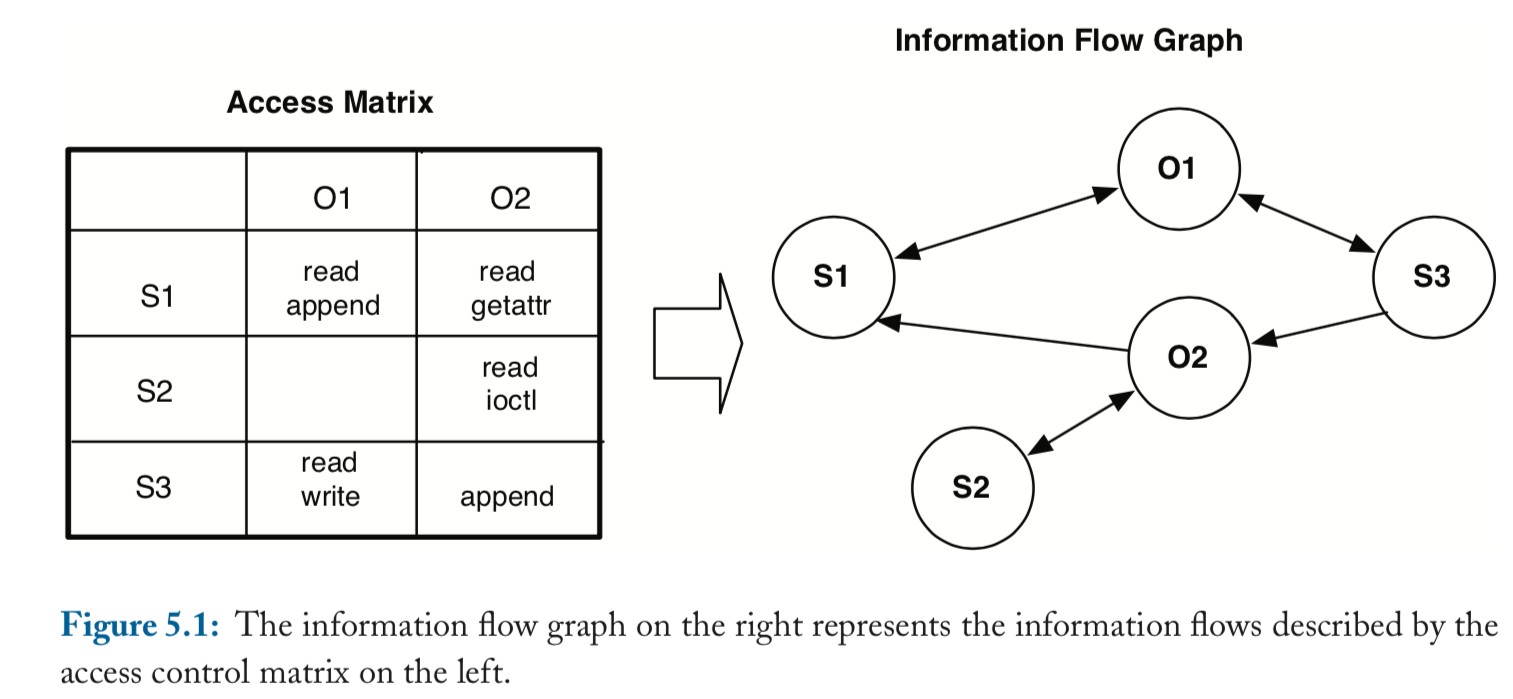
\includegraphics[width=\textwidth]{img/information-flow-graph}
    \\
    Trent Jaeger: Operating System Security, Chapter 5. Verifiable Security Goals
  \end{center}
\end{frame}

\begin{frame}{The Bell-LaPadula Model}
  \begin{itemize}
    \item focuses on confidentiality (not including integrity)
    \item military and governmental
    \item top secret, secret, confidential, unclassified
    \item low cannot read from high (read down)
    \item high cannot write to low (write up)
    \item Trusted Subjects transfer from high to low
  \end{itemize}
\end{frame}

\begin{frame}{Biba Integrity Model}
  \begin{itemize}
    \item focused on integrity: prevent modification and corruption
    \item povestea cu limbile
    \item high cannot read from low (read up)
    \item low cannot write to high (write down)
  \end{itemize}
\end{frame}

\begin{frame}{Clark Wilson Integrity Model}
  \begin{itemize}
    \item focused on integrity
    \item authenticated principal (user), set of programs (TP), data items
    \item certification rules and enforcement rules
  \end{itemize}
\end{frame}

\begin{frame}{Covert Channels}
  \begin{itemize}
    \item side channels
    \item implicit communication channels
    \item communication outside the control of the reference monitor
    \item storage channel (can theoretically be completely removed), timing channel (cannot be completely removed)
    \item fuzzy time (randomizing behavior)
    \item non-interference
  \end{itemize}
\end{frame}

\section{Decentralized Information Flow Control}

\begin{frame}{Decentralized Information Flow Control}
  \begin{itemize}
    \item share data with distrusted code
    \item suited for complex systems for a centralized model is unattainable
    \item labels annotate code
    \item checking can be done by compiler, similar to type checking
  \end{itemize}
\end{frame}

\begin{frame}[fragile]{Implicit Information Flow}
  \begin{verbatim}
x := 0
if b then
    x := 1
end
  \end{verbatim}
\end{frame}

\begin{frame}{Language-level Information Flow Control}
  \begin{itemize}
    \item povestea cu limbile
  \end{itemize}
\end{frame}

\begin{frame}{OS-level}
  \begin{itemize}
    \item Asbestos, HiStar, Fume
  \end{itemize}
\end{frame}

\section{Fine-grained Dynamic Information Tracking}

\begin{frame}{Fine-grained Tracking}
  \begin{itemize}
    \item povestea cu limbile
  \end{itemize}
\end{frame}

\begin{frame}{Taint Analysis}
  \begin{itemize}
    \item povestea cu limbile
  \end{itemize}
\end{frame}

\begin{frame}{Perl Taint Tracking}
  \begin{itemize}
    \item povestea cu limbile
  \end{itemize}
\end{frame}

\begin{frame}{Taint Analysis Solutions}
  \begin{itemize}
    \item povestea cu limbile
  \end{itemize}
\end{frame}

\section{Summary}

\begin{frame}{Summary}
  \begin{itemize}
    \item povestea cu limbile
  \end{itemize}
\end{frame}

\begin{frame}{Keywords}
  \begin{columns}
    \begin{column}{0.5\textwidth}
      \begin{itemize}
        \item TODO
      \end{itemize}
    \end{column}
    \begin{column}{0.5\textwidth}
      \begin{itemize}
        \item TODO
      \end{itemize}
    \end{column}
  \end{columns}
\end{frame}

\begin{frame}{Resources}
  \begin{itemize}
    \item Pin
    \item shell-storm
    \item Perl taint tracking
    \item Triton
    \item \url{https://web.cecs.pdx.edu/~apt/cs491/collins_presentation.html}
    \item \url{https://www.cs.uoregon.edu/research/summerschool/summer03/lectures/flow.pdf}
    \item \url{http://www.csc.kth.se/utbildning/kth/kurser/DD2460/Slides/trans_slides_SSS-part-3_lect-1_information-flow-security.pdf}
  \end{itemize}
\end{frame}

\begin{frame}{References}
  \begin{itemize}
    \item Trent Jaeger: Operating System Security
    \item Bell LaPadula
    \item Biba and Clark Wilson:
    \item Andrew Myers
    \item Jif
    \item Asbestos
    \item HiStar
    \item Flume
    \item Aquifer
    \item Weir
    \item TaintBochs
    \item Panorama
    \item TaintDroid
    \item FlowDroid
    \item Dorothy Denning: A Lattice Model of Secure Information Flow
  \end{itemize}
\end{frame}

\end{document}
